\documentclass[convert={size=500x1300,outext=.jpg},class=minimal,border=0mm]{standalone}
\usepackage{tikz}
\usetikzlibrary{backgrounds}
\usetikzlibrary{patterns}
\begin{document}
\begin{tikzpicture}[ show background rectangle, background rectangle/.style={fill=white} ]

	\tikzstyle{fractional}=[fill=red!40]
	\tikzstyle{integer}=[fill=blue!15]
	\tikzstyle{sign}=[fill=purple!15]

	%FPF=(-3,-34)
	\draw (2.000000,0.000000) rectangle ++(1,1) [fill=red!40,] node[midway] {0};
	\draw (3.000000,0.000000) rectangle ++(1,1) [fill=purple!15,] node[midway] {1};
	\draw (4.000000,0.000000) rectangle ++(1,1) [fill=purple!15,] node[midway] {1};
	\draw (5.000000,0.000000) rectangle ++(1,1) [fill=purple!15,] node[midway] {0};
	\draw (6.000000,0.000000) rectangle ++(1,1) [fill=purple!15,] node[midway] {0};
	\draw (7.000000,0.000000) rectangle ++(1,1) [fill=purple!15,] node[midway] {0};
	\draw (8.000000,0.000000) rectangle ++(1,1) [fill=purple!15,] node[midway] {1};
	\draw (9.000000,0.000000) rectangle ++(1,1) [fill=purple!15,] node[midway] {1};
	\draw (10.000000,0.000000) rectangle ++(1,1) [fill=purple!15,] node[midway] {0};
	\draw (11.000000,0.000000) rectangle ++(1,1) [fill=purple!15,] node[midway] {1};
	\draw (12.000000,0.000000) rectangle ++(1,1) [fill=purple!15,] node[midway] {0};
	\draw (13.000000,0.000000) rectangle ++(1,1) [fill=purple!15,] node[midway] {1};
	\draw (14.000000,0.000000) rectangle ++(1,1) [fill=purple!15,] node[midway] {0};
	\draw (15.000000,0.000000) rectangle ++(1,1) [fill=purple!15,] node[midway] {0};
	\draw (16.000000,0.000000) rectangle ++(1,1) [fill=purple!15,] node[midway] {1};
	\draw (17.000000,0.000000) rectangle ++(1,1) [fill=purple!15,] node[midway] {1};
	\draw (18.000000,0.000000) rectangle ++(1,1) [fill=purple!15,] node[midway] {1};
	\draw (19.000000,0.000000) rectangle ++(1,1) [fill=purple!15,] node[midway] {1};
	\draw (20.000000,0.000000) rectangle ++(1,1) [fill=purple!15,] node[midway] {1};
	\draw (21.000000,0.000000) rectangle ++(1,1) [fill=purple!15,] node[midway] {1};
	\draw (22.000000,0.000000) rectangle ++(1,1) [fill=purple!15,] node[midway] {0};
	\draw (23.000000,0.000000) rectangle ++(1,1) [fill=purple!15,] node[midway] {1};
	\draw (24.000000,0.000000) rectangle ++(1,1) [fill=purple!15,] node[midway] {1};
	\draw (25.000000,0.000000) rectangle ++(1,1) [fill=purple!15,] node[midway] {1};
	\draw (26.000000,0.000000) rectangle ++(1,1) [fill=purple!15,] node[midway] {1};
	\draw (27.000000,0.000000) rectangle ++(1,1) [fill=purple!15,] node[midway] {1};
	\draw (28.000000,0.000000) rectangle ++(1,1) [fill=purple!15,] node[midway] {0};
	\draw (29.000000,0.000000) rectangle ++(1,1) [fill=purple!15,] node[midway] {0};
	\draw (30.000000,0.000000) rectangle ++(1,1) [fill=purple!15,] node[midway] {1};
	\draw (31.000000,0.000000) rectangle ++(1,1) [fill=purple!15,] node[midway] {1};
	\draw (32.000000,0.000000) rectangle ++(1,1) [fill=purple!15,] node[midway] {1};
	\draw (33.000000,0.000000) rectangle ++(1,1) [fill=purple!15,] node[midway] {1};
	\draw[black,fill] (0,0.000000) circle [radius=0.1cm];


\end{tikzpicture}
\end{document}